The user should be able to make a taxi request from the web application and the mobile application. The reservation must contain the origin and the destination of the ride. The user has to specify also the date and hour of the reservation. If the values for the reservation are valid, the user can send the request to the system. Then the user will receive a notification with the taxi identifier.

\subparagraph{Use case}
\noindent
    \begin{center}
        \begin{longtable}{| l | p{0.6\textwidth} |}
            \hline
            Actor & Passenger \\
            \hline
            Goal & Goal~\ref{g-reserve}
            \\
            \hline
            Input condition & A user chooses to make a taxi reservation from his account page; \\
            \hline
            Event Flow & 
                \begin{enumerate}
                	\item The user makes a request of a taxi inserting all the required information in the application page;
                	\item The user sends the reservation to the system using the "Make reservation" button.
            	\end{enumerate}
            \\
            \hline
            Output condition & The user receives the confirmation of the reservation 10 minutes before the time chosen during the request making. \\
            \hline
            Exception & 
            \begin{itemize}
                \item There are no available taxi in the area;
                \item When ten taxi drivers refuse the reservation, it is canceled.
            \end{itemize} \\
            \hline
        \end{longtable}
    \end{center}

\subparagraph{Functional requirements}
\noindent
	\begin{itemize}
		\item The origin and the destination must be valid [View assumptions]. They must be within 10Km from the city boundaries.
		\item If the GPS is available the user can use the current position as origin of the ride.
		\item The date and the time of the reservation must be valid values.
		\item The system does not allow reservation after 24 hours from the current system time.
		\item The system sends a notification to the user 10 minutes before the hour chosen by the user for the ride. The notification contains the taxi identifier.
	\end{itemize}
	
\begin{figure}[H]
    \centering
    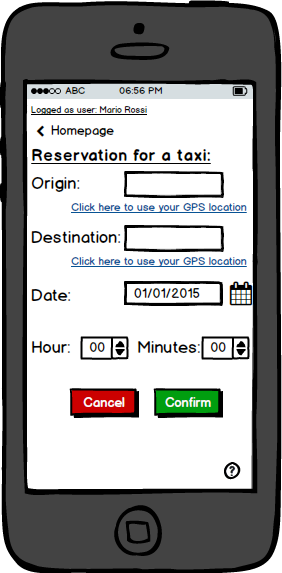
\includegraphics[width=5cm]{./Mockups/Reservation.png}
    \caption{Reservation making page}
\end{figure}
